% @Author: Your name
% @Date:   2017-08-17 15:16:16
% @Last Modified by:   Your name
% @Last Modified time: 2023-03-27 18:40:11
%%    2009/03/12 v1.0 GAUBM Vorlage f�r Aschlussarbeiten Physik
%% Template fuer Bachelor- und Masterarbeiten
%% an der Fakultaet fuer Physik (c) Thomas Pruschke der GA Universit�t
%% Verbesserungsvorschlaege bitte an studiendekanat@physik.uni-goettingen.de
%%
%% Benoetigte Pakete: datenumber
%%

%%%%%%%%%%%%%%%%%%%%%%%%%%%%%%%%%%%%%%%%%%%%%%%%%%%%%%%%%%%%%%%%%%%%%%
%%%%%%%%%% Bitte vor dem Veraendern diese Datei umbenennen! %%%%%%%%%%
%%%%%%%%%%%%%%%%%%%%%%%%%%%%%%%%%%%%%%%%%%%%%%%%%%%%%%%%%%%%%%%%%%%%%%

%% scrbook - Ersatz f�r LaTeX book Klasse aus dem KOMA Script
%% Moegliche Optionen: diejenigen der Klasse scrbook ausser titlepage

%% deutsche Arbeit:
\documentclass[bachelor,       %% Typ der Arbeit: bachelor oder master
               twoside,        %% zweiseitiges Layout
               BCOR10mm,       %% Bindekorrektur 10 mm
%               liststotoc,nomtotoc,bibtotoc, %% Aufnahme der div. Verzeichnisse
                                              %% ins Inhaltsverzeichnis
%               english,ngerman, %% Alternativspr. Englisch, Dokumentspr. Deutsch
                ngerman,english  %% Alternativspr. Deutsch, Dokumentspr. Englisch
%               final,          %% Endversion; draft fuer schnelles Kompilieren
               ]{GAUBM}
\usepackage{graphicx}
\usepackage{caption}
\usepackage{subcaption}
\usepackage{csquotes}
\usepackage[nohyperlinks, printonlyused, withpage, smaller]{acronym}
\usepackage{setspace}  %% Zur Setzung des Zeilenabstandes
\usepackage{babel}     %% Sprachen-Unterstuetzung
\usepackage{calc}      %% ermoeglicht Rechnen mit Laengen und Zaehlern
\usepackage[T1]{fontenc}       %% Unterstutzung von Umlauten etc.
\usepackage[latin1]{inputenc}  %% 
%% in aktuellem Linux & MacOS X wird standardmaessig UTF8 kodiert!
%\usepackage[utf8]{inputenc}    %% Wenn latin1 nicht geht ...

\usepackage{amsmath,amssymb} %% zusaetzliche Mathe-Symbole

\usepackage{lmodern} %% type1-taugliche CM-Schrift als Variante zur
                     %% "normalen" EC-Schrift
%% Paket fuer bibtex-Datenbanken
\usepackage[comma,numbers,sort&compress]{natbib}
\bibliographystyle{plainnat}

\newcommand{\tabheadfont}[1]{\textbf{#1}} %% Tabellenkopf in Fett
\usepackage{booktabs}                      %% Befehle fuer besseres Tabellenlayout
\usepackage{longtable}                     %% umbrechbare Tabellen
\usepackage{array}                         %% zusaetzliche Spaltenoptionen

%% umfangreiche Pakete fuer Symbole wie \micro, \ohm, \degree, \celsius etc.
\usepackage{textcomp,gensymb}

%\usepackage{SIunits} %% Korrektes Setzen von Einheiten
\usepackage{units}   %% Variante fuer Einheiten

%% Hyperlinks im Dokument; muss als eines der letzten Pakete geladen werden
\usepackage[pdfstartview=FitH,      % Oeffnen mit fit width
            breaklinks=true,        % Umbrueche in Links, nur bei pdflatex default
            bookmarksopen=true,     % aufgeklappte Bookmarks
            bookmarksnumbered=true  % Kapitelnummerierung in bookmarks
            ]{hyperref}

%% Weiter benoetigte Pakete: datenumber
%% Falls dieses Paket nicht in der Installation vorhanden ist,
%% kann es von der Seite mit diesem Template heruntergeladen werden
%% und in einem LaTeX bekanntem Verzeichnis installiert werden (notfalls
%% dem Verzeichnis mit der Arbeit).
\begin{document}
%%
%%                   Ab hier muessen die Anpassungen geschehen
%%
%% Hier den eigenen Namen einsetzen
\ThesisAuthor{Justus}{Multhaup}
%% Hier den Geburtsort einsetzen
\PlaceOfBirth{Boffzen}
%% Titel Arbeit. Das erste Argument ist der deutsche, das zweite der
%% englische Titel.
\ThesisTitle{Teilchensimulationen von Polymermischungen in begrenzten Geometrien mit zeitabh\"angigen Randbedingungen}{Particle simulations of polymer mixtures in confined geometries with time dependent boundary conditions}
%% Erst- und Zweitgutacher/in
%% Ist der/die Betreuer/in nicht identisch mit dem/r Erstgutachter/in,
%% muss diese/r als optionales Argument angegeben werden.
\FirstReferee{Prof. Dr. Marcus M\"uller}
\Institute{Institut f\"ur Theoretische Physik}
\SecondReferee{Prof. Dr. Stefan Klumpp}
%% Beginn und Ende des Anfertigungszeitraumes
\ThesisBegin{1}{4}{2009}
\ThesisEnd{15}{7}{2009}
%% DO NOT TOUCH THESE LINES!!!!
\frontmatter
\maketitle
\cleardoublepage


%% Ende des Vorspanns
\cleardoublepage
%% Ab hier 1 1/2 facher Zeilenabstand (durch setspace-Paket)
\onehalfspacing
%% Erzeugt Inhaltsverzeichnis
\tableofcontents

%% Hier kann man seine Bezeichnungsweisen erklaeren. Falls nicht
%% benoetigt, bis einschliesslich \end{nomenclature} auskommentieren
% \begin{nomenclature}
% %% Fuer die Berechnung der Spaltenbreiten muss \usepackage{calc}
% %% geladen sein!
% \section*{Lateinische Buchstaben}
% \noindent
% \begin{longtable}[l]{p{0.2\textwidth}p{0.7\textwidth-6\tabcolsep}p{0.1\textwidth}}
%   \tabheadfont{Variable}&\tabheadfont{Bedeutung}&\tabheadfont{Einheit}\\\midrule\endhead
%   $A$ & Querschnittsfl"ache & $\unit{m^2}$\\
%   $c$ & Geschwindigkeit & $\unitfrac{m}{s}$
% \end{longtable}
% \section*{Griechische Buchstaben}
% \begin{longtable}[l]{p{0.2\textwidth}p{0.7\textwidth-6\tabcolsep}p{0.1\textwidth}}
%   \tabheadfont{Variable}&\tabheadfont{Bedeutung}&\tabheadfont{Einheit}\\\midrule\endhead
%   $\alpha$  & Winkel & $\unit{\degree}$; --\\
%   $\varrho$ & Dichte & $\unitfrac{kg}{m^3}$
% \end{longtable}
% \section*{Indizes}
% \begin{longtable}[l]{p{0.2\textwidth}p{0.8\textwidth-4\tabcolsep}}
%   \tabheadfont{Index}&\tabheadfont{Bedeutung}\\\midrule\endhead
%   m & Meridian\\
%   $r$ & Radial
% \end{longtable}
% \section*{Acronyms}
% \begin{longtable}[l]{p{0.2\textwidth}p{0.8\textwidth-4\tabcolsep}}
%   \tabheadfont{Acronym}&\tabheadfont{Meaning}\\\midrule\endhead
%   SOMA & SOft coarse-grained
%   Monte-Carlo Acceleration\\
%   SCF & self-consistent field\\
%   SCMF & single chain in mean field\\
% \end{longtable}
% \begin{acronym}[EuGH]
%   \acro{eugh}[EuGH]{Europäischer Gerichtshof}
%   \acro{eu}[EU]{Europäische Union} 
%   \end{acronym}
% \end{nomenclature}
%% \listoftables und \listoffigures sollten nur bei genuegender Anzahl Tabellen
%% verwendet werden
%\listoffigures
%\listoftables

\mainmatter   %% Anfang Hauptteil

\chapter{Introduction}

Polymers are highly versatile macromolecules composed of repeating units called monomers. Their importance for life on earth cannot be overstated, they are involved in countless chemical reactions in the human body and form the backbone of proteins and DNA. They are applied almost everywhere in modern society, ranging from simple packaging materials to highly sophisticated materials used in aerospace engineering. This is owed to their vast range of unique physical properties, such as high elasticity, flexibility and durability. When creating novel materials with very precise features, understanding how polymers form and interact with one another is essential.\\
One important class of polymers is the so-called homopolymer, which is made of a single type of monomer unit, for example, polyethylene. Copolymers, in contrast, consist of two or more different types of monomer units. These monomer units may arrange into blocks, so that the resulting polymer can be viewed as a concatenation of homopolymers of different types, this is then called a block-copolymer. One of the most interesting and extensively studied properties of copolymers is their ability to self-assemble into microphases \cite{leibler1980theory}. One of the most important tools in understanding the mechanisms behind this microphase-separation, and many other interesting properties, is the use of computer simulations. These include particle-based molecular dynamics (MD), Monte-Carlo (MC) methods as well as continuum-model-based and hybrid methods \cite{Shuanhu2017}. Particle-based simulations accurately model small-scale phenomena. However, despite rapid advancements in computer technology and high parallelizability, they are too computationally expensive to simulate large systems and therefore capture macroscale phenomena. Continuum models, on the other hand, are less computationally expensive, but at the cost of a lower accuracy on the microscale. On the mesoscale, e.g. the orientation of cylindrical mesophases upon solvent evaporation \cite{Dreyer22}, good agreement between the two types of models was observed. To evaluate the performance of continuum models on small-length scales, it is necessary to compare them to established particle-based models. One way to do this is to consider a simulation box in a particle-based simulation as a small section from a large continuum-model-based simulation. The dynamics are then driven by extracting the time evolution of the density fields at the boundaries from the continuum-simulation and applying them in the particle-based simulation, e.g. employing non-periodic boundary conditions. However, dictating the boundary densities in particle-based simulations is not a trivial task. One option is the use of external fields or the umbrella sampling method \cite{glenn74}, although this has the large drawback that the number of particles in the simulation box remains constant, while in the continuum simulation particles can enter and leave the section at any time. An alternative is to employ conversion zones at the boundaries, in which molecules are converted to different types, mimicking particle exchange with the surrounding. If the densities are defined on a discretized grid, this leads to an optimization problem in which the ideal configuration of molecule types needs to be found, such that the mean squared deviation from the target density is minimized. \\
In this study, as a first step towards boundary-driven particle simulations, the dynamics of noninteracting homopolymers are investigated. Specifically, a system is pushed away from equilibrium by introducing conversion zones at the boundary regions of the simulation box. This results in a diffusion-driven current and allows the calculation of the collective diffusion coefficient of the system. To this end, the SOft coarse-grained Monte-Carlo Acceleration (SOMA) \cite{Schneider_soma} software package based on the single chain in mean field algorithm (SCMF) \cite{Daoulas06} is employed.



\chapter{Theory}

\section{Polymeric mixtures}
Polymer mixtures consist of two or more chemically different polymer types. The mechanical and thermodynamic properties can vary greatly with several factors such as composition, molecular weight and interactions between the polymers. This makes them desirable for manufacturing materials with tailored properties.\\
If the composition is uniform everywhere, then the mixture is called homogeneous. In this case, the properties do not change throughout the mixture. In a heterogeneous mixture, in contrast, the composition is non-uniform, leading to visible boundaries which may have very different properties. This phenomenon is also called macro-phase separation. From an entropic viewpoint, mixing is always favored. However, energetic interactions between polymers can either favor or suppress mixing. Whether a mixture is homogeneous or heterogeneous therefore depends on the balance between entropy and energy \cite[S. 137]{Rubin03}.           

\subsection{Flory Huggins Theory}

Whether mixing or phase separation will be favored can be predicted by determining the free energy change associated with mixing the components. This free energy change can be computed within the lattice model developed by Flory and Huggins \cite{Flory42}. Within the Flory-Huggins framework, no volume change is assumed upon mixing. With this assumption, it is convenient to represent the system on a lattice. The lattice site volume $v_0$ corresponds to the smallest molecular unit and every macromolecule takes up one or multiple lattice sites. Consider a binary mixture with $n_A$ polymers of species A and chain length $N_A$ and $n_B$ polymers of species B and chain length $N_B$. Let the total number of polymers be $n=n_A+n_B\,.$ The free energy of mixing per lattice site $\Delta F_{mix}$ is then given by the Flory-Huggins equation of polymer solutions \cite[S. 143]{Rubin03}:

\begin{align}
  \frac{\Delta F_{mix}}{k_BT}=\frac{\phi}{N_A}\ln\phi+\frac{1-\phi}{N_B}\ln(1-\phi)+\chi\phi(1-\phi)\,.
\end{align}

Here, $\phi=\frac{n_AN_A}{n_AN_A+n_BN_B}$ is the monomer fraction of species A, $k_B$ is the Boltzmann constant, $T$ is the system temperature and $\chi$ is the Flory interaction parameter which characterizes the interaction between different polymer species and can be obtained from experiments. A positive value of $\chi$ opposes mixing while a negative value promotes it, knowing the value of $\chi$, therefore, allows a qualitative prediction of the phase separation behavior. Note that so far, no space dependency of $\phi$ has been assumed. In the following discussion, a symmetric mixture with $N_A=N_B=N$ is assumed. To fully capture the complexity of the system, the Flory-Huggins model has to be extended to include spatial variations of $\phi$, which gives rise to the de Gennes-Flory-Huggins free energy functional  \cite{deGennes80, Reister02}:


\begin{align}
  \frac{F[\phi]R_e^3}{k_BT\sqrt{\bar N}}=\int \mathrm{d}^3\mathbf{r}\left\{\phi\ln\phi+(1-\phi)\ln(1-\phi)+\chi N\phi(1-\phi)+k(\phi)[\nabla\phi]^2\right\}\,.
  \label{eq:flory_fctl}
\end{align}

Here, $R_e^2=(N-1)b^2$ is the mean squared end-to-end distance of the polymer in the absence of non-bonded interactions, where $b$ is the statistical segment length, and $\bar N=\left(nR_e^3/V\right)^2$ is the invariant degree of polymerization of the system with volume $V$. The latter is a measure of the number of neighboring chains a chain interacts with. The term proportional to $[\nabla\phi]^2$ is added to the free energy density to ensure that unphysical, sharp changes in the local densities are penalized. The precise form of $k(\phi)$ depends on the strength of the parameter $\chi\,$. For small $\chi N\lesssim 10.5\,,$ one considers the \textit{weak segregation limit} (WSL). For very large $\chi N\gtrsim300\,,$ the \textit{strong segregation limit} (SSL) holds. In these two limits, the prefactor $k$ takes the form \cite{Reister02}:

\begin{align}
  k_\mathrm{WSL}=\frac{R_e^2}{36\phi(1-\phi)}\,;\qquad k_\mathrm{SSL}=\frac{R_e^2}{18\phi(1-\phi)}\,.
\end{align}


\section{Collective diffusion}

Consider a binary mixture of polymers with $N_A=N_B=N\,$. Since the number of monomers in the system is constant, the continuity equation holds:

\begin{align}
  \frac{\partial\phi}{\partial t}+\nabla\cdot\mathbf{J}=0\,.
  \label{eq:conti}
\end{align}

Here, $\mathbf{J}$ is the local current of species A. Near equilibrium, one postulates a linear relation between $\mathbf J$ and the local chemical potential difference $\mu$ \cite{deGennes80}:


\begin{align}
    \mathbf J(\mathbf{r})=-\int_V\frac{\Lambda(\mathbf{r}, \mathbf{r'})}{k_BT}\nabla '\mu(\mathbf{r'})\text d \mathbf{r'}\,.
    \label{eq:current}
\end{align}

The Onsager coefficient $\Lambda(\mathbf{r}, \mathbf{r'})$ relates the force acting on a monomer at position $\mathbf{r'}$ due to the gradient of chemical potential to the density at position $\mathbf{r}\,$. In the literature, this nonlocal coupling is often dropped for the sake of computational efficiency \cite{Fraaje97,deGennes80,Binder83}. This leads to a simple version of the Onsager coefficient that will be derived in the following. 

%%  Derivation in Binder paper

% Following the discussion in the appendix of \cite{Binder83}, a continuity equation can be written down for each type individually:

% \begin{align}
%   \frac{\partial\phi_A}{\partial t}+\nabla\cdot\mathbf{J_A}=0\,; \qquad \frac{\partial\phi_B}{\partial t}+\nabla\cdot\mathbf{J_B}=0\,.
%   \label{eq:conti_ab}
% \end{align}

% With the additional assumption of incompressibility, e.g. $\rho(\mathbf{r},t)\equiv\phi_A(\mathbf{r},t)+\phi_B(\mathbf{r},t)=1$ everywhere for all times, the continuity equation for the total density $\rho$ separates into two distinct equations:

% \begin{align}
%   \frac{\partial}{\partial t}(\phi_A+\phi_B)=0\,; \qquad \nabla\cdot (\mathbf{J_A}+\mathbf{J_B})=0  \,.
% \end{align}

% This implies that $\mathbf{J_A}=-\mathbf{J_B}\,,$ which simply reflects the condition of incompressibility: for a bead of type A to move, a bead of type B has to take its place and vice-versa. The Onsager relations are then
% \begin{subequations}
%   \begin{align}
%     \mathbf{J_A}&=-\frac{\Lambda_{\mathrm{AA}}}{k_BT}\nabla\mu_\mathrm A\,,\\
%     \mathbf{J_B}&=-\frac{\Lambda_{\mathrm{BB}}}{k_BT}\nabla\mu_\mathrm B\,,
%     \label{eq:current_onsager}
%   \end{align}
% \end{subequations}


% where $\Lambda_\mathrm{AA}$ and $\Lambda_\mathrm{BB}$ are the diagonal elements of the matrix of Onsager coefficients, which is assumed to be diagonal. Since $\mu_\mathrm A$ and  $\mu_\mathrm B$ are not independent variables, their difference $\Delta\mu=\mu_\mathrm A-\mu_\mathrm B$ is considered instead. The goal is now to relate $\Delta\mu$ to the current $\mathbf J(\mathbf r,t)=\mathbf {J_A}(\mathbf r,t)=-\mathbf {J_B}(\mathbf r,t)\,.$ From \eqref{eq:current_onsager}, it is easily seen that

% \begin{align}
%   \nabla(\mu_\mathrm A-\mu_\mathrm B)&=-k_BT\left (\mathbf{J_A}\Lambda_{\mathrm{AA}}^{-1} - \mathbf{J_B}\Lambda_{\mathrm{BB}}^{-1}\right )\nonumber\\
%   &=-k_BT\left (\Lambda_\mathrm{AA}^{-1}+\Lambda_\mathrm{BB}^{-1}\right )\mathbf{J}
% \end{align}

% and therefore

% \begin{align}
%   \mathbf J=-\frac{1}{k_BT}\left (\Lambda_\mathrm{AA}^{-1}+\Lambda_\mathrm{BB}^{-1}\right )^{-1}\nabla(\mu_\mathrm A-\mu_\mathrm B)\,.
% \end{align}

% The Onsager coefficient that relates $\mathbf{J}$ to the local chemical potential difference is identified as $\Lambda^{-1}=\Lambda_\mathrm{AA}^{-1}+\Lambda_\mathrm{BB}^{-1}\,.$ By relating the currents in \eqref{eq:current_onsager} to the single chain diffusion coefficients $D_A$ and $D_B\,,$ the Onsager coefficients may be identified as $\Lambda_\mathrm{AA}=N_AD_A\phi$ and $\Lambda_\mathrm{BB}=N_BD_B(1-\phi)\,.$ For a symmetric mixture with $N_A=N_B\equiv N $ and $D_A=D_B\equiv D\,,$ the Onsager coefficient corresponding to $\Delta\mu$ becomes


% \begin{align}
%   \Lambda=DN\phi(\mathbf{r})(1-\phi(\mathbf{r}))\,.
%   \label{eq:onsager}
% \end{align}


% This result has also been derived by de Gennes \cite{deGennes80}.\\


%% Alternative derivation in de Gennes paper


Following the discussion in the appendix of \cite{deGennes80}, consider a mixture of non-interacting chains with densities $\phi_A$ and $\phi_B\,.$ The currents are simply given by Fick's law of Diffusion:

\begin{align}
  \mathbf{J_A}=-D_\mathrm A\nabla\phi_\mathrm A\,; \qquad \mathbf{J_B}=-D_\mathrm B\nabla\phi_\mathrm B\,.
\end{align}

The chemical potential per monomer for an ideal gas of A chains with concentration $\phi_A/N$ is:

\begin{align}
  \frac{\mu_\mathrm A}{k_BT}=\frac{\partial}{\partial\phi_\mathrm A}\left(\frac{\phi_A}{N}\ln\frac{\phi_A}{N}+\mathrm{const}\right)=N^{-1}\ln\phi_\mathrm A +\mathrm{const}\,,
\end{align}

and similarly for $\mu_\mathrm B\,.$ The currents may then be related to the chemical potential by writing:
\begin{align}
  \mathbf{J}_i=-\Lambda_i\nabla\mu_i\,; \qquad \Lambda_i=D_iN\phi_i^{-1}\,.
  \label{eq:current_ideal}
\end{align}

Incompressibility, e.g. $\phi_\mathrm A+\phi_\mathrm B=1\,,$ is enforced by introducing an additional repulsive potential $U$ to the chemical potential, so \eqref{eq:current_ideal} is modified to:

\begin{subequations}
  \begin{align}
    \mathbf{J_A}&=-\Lambda_\mathrm A\nabla [(\mu_\mathrm A + U)/k_BT]\,,\\
    \mathbf{J_B}&=-\Lambda_\mathrm B\nabla [(\mu_\mathrm B + U)/k_BT]\,.
  \end{align}
  \label{eq:current_onsager}
\end{subequations}

Due to the incompressibility, the currents must have zero divergence, which imposes $\mathbf{J_A}+\mathbf{J_B}=0\,.$ From this condition, $U$ can be calculated explicitly:

\begin{align}
  U=(\Lambda_\mathrm A\mu_\mathrm A+\Lambda_\mathrm B\mu_\mathrm B)/(\Lambda_\mathrm A+\Lambda_\mathrm B)\,.
\end{align}

Since one of the currents is redundant, write $\mathbf{J}=\mathbf{J_A}\,.$ From \eqref{eq:current_onsager}, we get:

\begin{align}
  \mathbf J=-\Lambda\nabla(\mu_\mathrm A - \mu_\mathrm B)\equiv -\Lambda\nabla\mu\,,
\end{align}

where $\Lambda=\Lambda_\mathrm A\Lambda_\mathrm B/(\Lambda_\mathrm A+\Lambda_\mathrm B)$ and $\mu$ is the exchange chemical potential. For $D_\mathrm A=D_\mathrm B\equiv D\,,$ this yields:

\begin{align}
  \Lambda=DN\phi(\mathbf{r})(1-\phi(\mathbf{r}))\,.
  \label{eq:onsager}
\end{align}


It should be noted that, in the general case, the single-chain dynamics will affect the collective dynamics in a more complex way that is expressed by including the pair-correlation functions of A and B in the Onsager coefficient \cite{Reister02}. 

\chapter{Simulation technique}

To simulate the collective dynamics, a coarse-grained model of the polymers is employed. Within this model, several monomeric repeat units are grouped into an effective interaction center, called \textit{bead}, which allows for an efficient numerical implementation. Nevertheless, in this thesis, the terms \enquote{bead} and \enquote{monomer} will be used interchangeably. A great variety of universal properties of polymeric materials on mesoscopic length scales is accurately captured by coarse-grained models \cite{Baschnagel03}.\\
The software package that is used for the numerical calculations, SOft coarse-grained Monte-Carlo Acceleration (SOMA) \cite{Schneider_soma}, uses a combination of a coarse-grained model and the single chain in mean field algorithm (SCMF) \cite{Daoulas06}, which is an extension of the self-consistent field (SCF) method. Unlike conventional SCF theory, the SCMF method includes fluctuation effects which are required to accurately describe certain systems and effects, e.g. dilute polymer solutions, the vicinity of phase transitions, or polymeric microemulsions \cite{Bates97, Mueller02, Schmid03}. Instead of calculating the interaction of a chain with all it's surrounding explicitly, the chains are subjected to fluctuating external fields which are frequently recalculated from the density distribution. The densities are defined on a cubic grid. The time evolution of the system is then performed by MC simulation, during which the external fields remain constant, this is called \textit{quasi-instantaneous field approximation}. The enormous benefit of this is that the chains are decoupled, making it possible to implement it effectively on parallel machines and leverage accelerators like Nivida GPUs. \cite{Schneider_soma}. Additionally, a Smart Monte-Carlo (SMC) scheme is employed that uses the strong bonded forces to propose a trial displacement resembling Brownian motion and produces Rouse-like dynamics \cite{Pangali78,Rossky78}.\\
While a full description of the SCMF equations can be found in \cite{Daoulas06}, and will be omitted here, it is important to note that, for AB diblock-copolymers, the interactions are fully described by three coarse-grained parameters: the average mean squared end-to-end distance $R_{e}^2$ of a chain in the absence of non-bonded interactions, the inverse thermal compressibility $\kappa_o N$ and the incompatibility between different bead types $\chi_o N$. The term \enquote{soft} in SOMA relates to the soft nature of the non-bonded interactions, which arises from the systematic coarse-graining and allows for an overlap of molecules \cite{Mueller11soft}.

\chapter{Collective diffusion of symmetric homopolymers}

\section{Reference system}

In this section, the collective diffusion properties of noninteracting homopolymers with $N_A=N_B=N$ and $\chi=0$ are investigated. As a reference system, a simulation box with 10000 polymers and dimensions $L_x\times L_y\times L_z=9.75\times3\times3\,R_e^3$ is considered with a spatial discretization of $\Delta L=0.125\,R_e\,$, so the invariant degree of polymerization is $\sqrt{\bar{N}}\approx 120\,$. Periodic boundary conditions are applied in the lateral $y$ and $z$ directions, whereas impenetrable walls are applied in the $x$ direction. Initially, the polymers are distributed homogeneously in the system. To stimulate diffusion, conversion zones are introduced close to the walls at $x<0.25\,R_e$ and $x>9\,R_e\,$. In each time step, if the center-of-mass coordinate $\mathbf r_{cm}$ of a polymer of type A lies in the conversion zone at $x<0.25\,R_e\,$, it is converted to type B with probability $p(A\rightarrow B)=r\phi(\mathbf r_{cm})$ \cite{Dreyer22}. Analogously, conversion from B to A takes place in the conversion zone at $x>9\,R_e$ at the same rate $r\,$. The total currents $\mathbf{J_A}$ and $\mathbf{J_B}$ are measured by tracking the number of polymer conversions. \\
The computation of the transport properties is complicated by boundary effects, such as a steep density drop close to the hard walls, which is of entropic origin. Furthermore, chains whose center of mass lies in the conversion zone may extend far beyond that zone. The range of these effects is approximated as $R_e$ and measurements are only taken in the region that is unaffected. 


\begin{figure}[h]
  \centering
  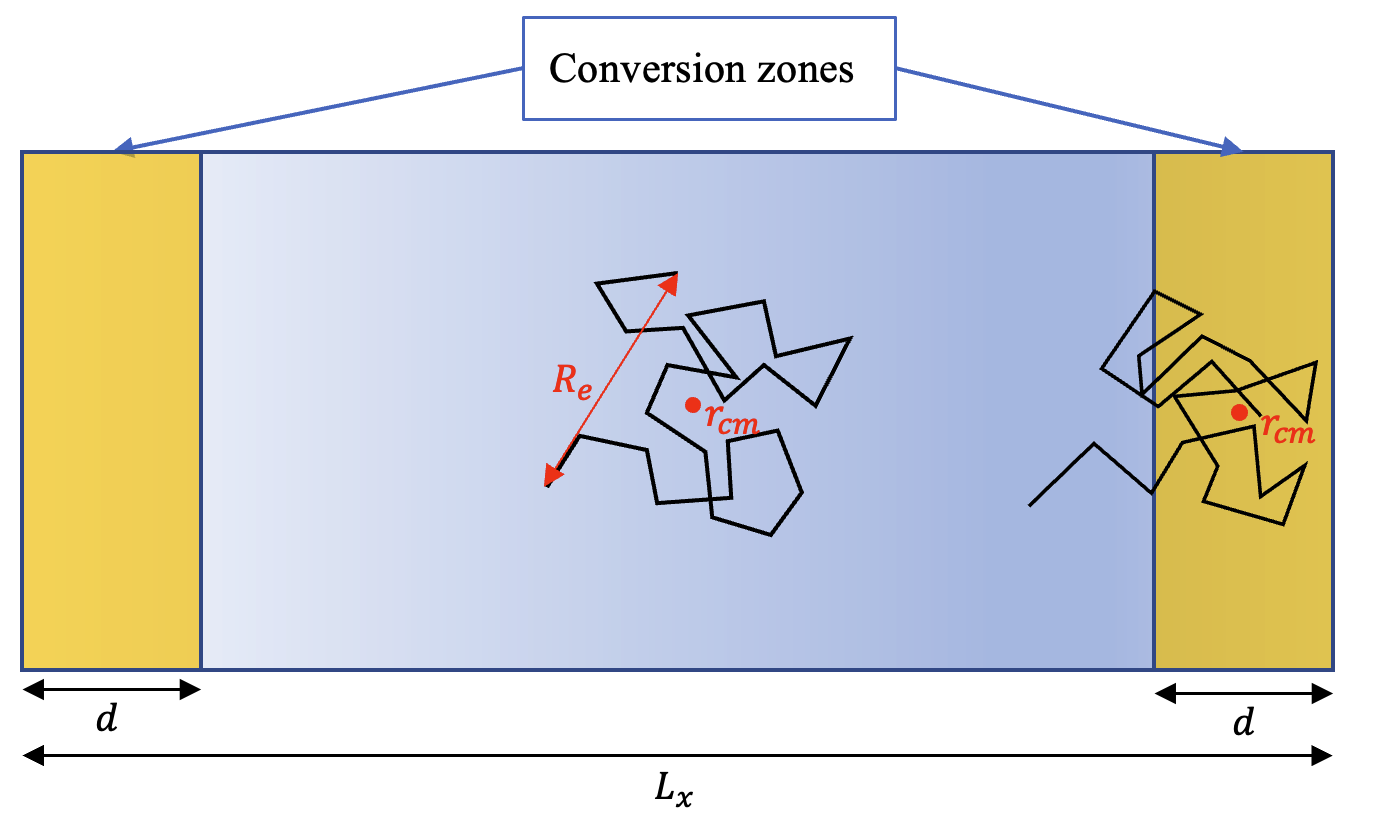
\includegraphics[width=0.7\linewidth]{figures/simulation_box.png}
  \caption{}
  \label{fig:simulation_box}
\end{figure}


\section{Collective diffusion coefficient}

It should be pointed out that the system can be described effectively in one dimension due to the periodic boundary conditions in the lateral directions. The chemical potential is obtained by taking the functional derivative $\frac{\delta F}{\delta\phi}$ of \eqref{eq:flory_fctl}. Since $\chi=0\,$, no phase separation occurs and the local density differences are entirely due to the dynamics. Assuming the WSL, the chemical potential becomes:


\begin{align}
  \frac{\mu R_e^3}{\sqrt{\bar N} k_BT}&=\ln\phi-\ln(1-\phi)-\frac{R_e^2}{18\phi(1-\phi)}\phi''\nonumber \\ &+\left[\frac{R_e^2(1-2\phi)}{36\phi^2(1-\phi)^2}\right]\phi'^2\,.
  \label{eq:mu_flory}
\end{align}

Here, $\phi'=\frac{\partial\phi}{\partial x}\,.$ The resulting chemical potential profile is shown in Figure \ref{fig:chemical_potential}.




\begin{figure}[h]
  \centering
  \begin{subfigure}[b]{0.45\textwidth}
      \centering
      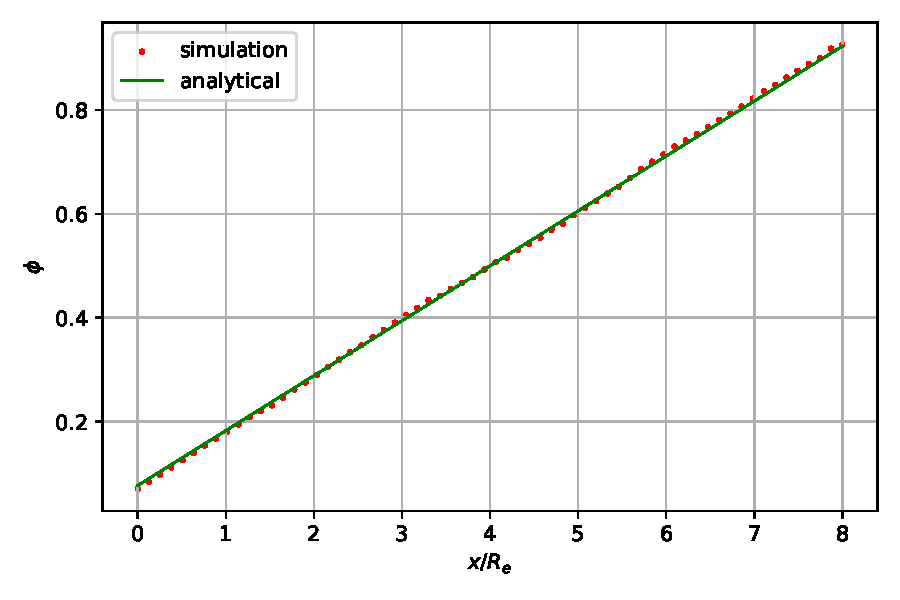
\includegraphics[width=\textwidth]{figures/density_coll_diff.pdf}
      \caption{}
      \label{fig:density_profile}
  \end{subfigure}
  \hfill
  \begin{subfigure}[b]{0.45\textwidth}
      \centering
      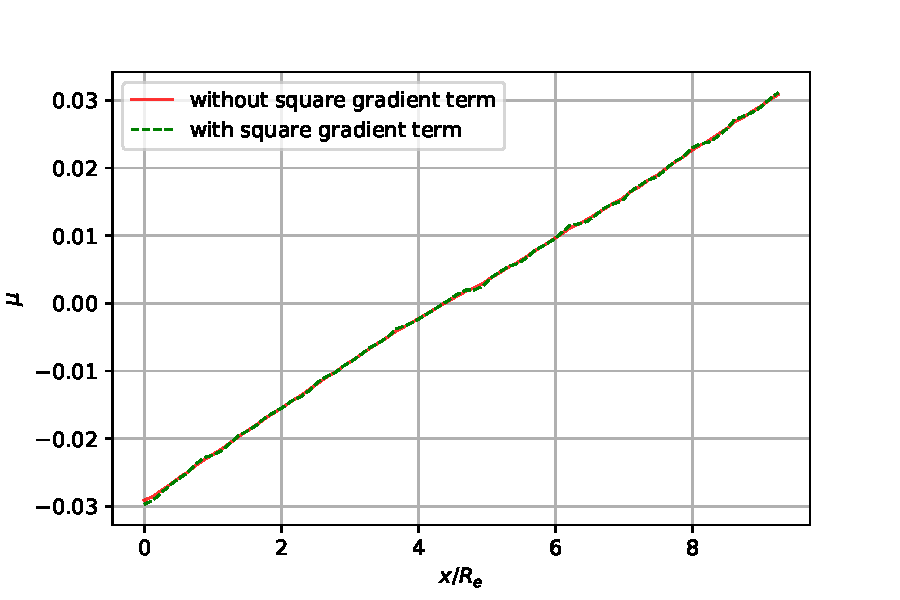
\includegraphics[width=\textwidth]{figures/mu_coll_diff.pdf}
      \caption{}
      \label{fig:chemical_potential}
  \end{subfigure}
     \caption{Density profile obtained from simulation (a) and chemical potential profile obtained from \eqref{eq:mu_flory} (b)  averaged over time, $y$ and $z$ for $r=1.0\,$. }
     \label{fig:mu_phi}
\end{figure}


In Figure \ref{fig:chemical_potential}, it can be seen that the terms arising from the square gradient term in the free energy do not contribute to the chemical potential, other than adding noise due to the numerical derivatives. Therefore, these terms prohibit an accurate numerical computation of the chemical potential gradient and thus the Onsager coefficient. In the subsequent discussion, these terms will be neglected. This approximation leads to a linear density profile, as derived below, which is also consistent with the simulation results shown in figure \ref{fig:density_profile}.

From \eqref{eq:current}, \eqref{eq:onsager} and \eqref{eq:mu_flory}, the current becomes:


\begin{align}
  J=-D\rho_0\phi'\,.
  \label{eq:current_a}
\end{align}



Here, $\rho_0=nN/V$ is the average bead density in the system. Together with \eqref{eq:conti}, this gives the well-known diffusion equation:
\begin{align}
  \frac{\partial\phi(\mathbf r, t)}{\partial t}-D\rho_0  \phi''=0\,.
  \label{eq:diffusion}
\end{align}

In the steady state, this simply yields $\phi''=0\,,$ so a linear density profile is obtained. From \eqref{eq:current_a} and the condition that $\phi(L_x/2)=0.5\,,$ which follows from the equal conversion rates, the density profile becomes:

\begin{align}
  \phi(x)=-\frac{J}{D\rho_0}x + \frac{1}{2} (1-L_x)\,.
  \label{eq:density_profile_ana}
\end{align}

To verify \eqref{eq:onsager}, the Onsager coefficient may also be obtained directly from the simulation results using \eqref{eq:current}. Again assuming local coupling and making use of \eqref{eq:mu_flory}, while neglecting the terms arising from the square gradient, one obtains:

\begin{align}
  \Lambda=-\frac{JR_e^3}{\sqrt{\bar N}\phi'}\phi(1-\phi).
  \label{eq:onsager_num}
\end{align}

\begin{figure}[h]
  \centering
  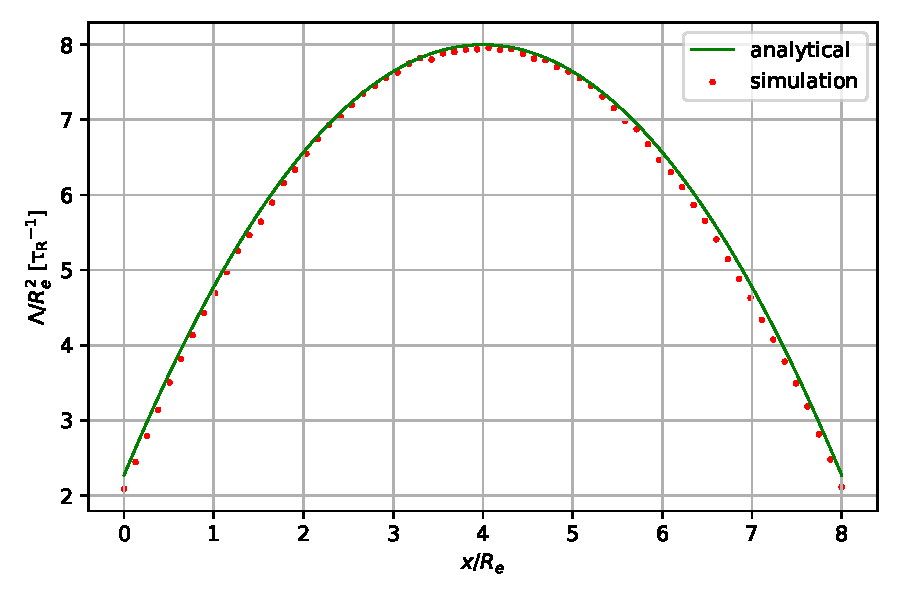
\includegraphics[width=0.7\linewidth]{figures/onsager_coll_diff.pdf}
  \caption{Onsager coefficient for $r=1.0\,$ averaged over time, $y$ and $z\,$. The analytical curve is obtained from \eqref{eq:onsager} and \eqref{eq:density_profile_ana}}, the numerical curve from \eqref{eq:onsager_num} and the density profile in \ref{fig:density_profile}. The diffusion constant $D$ and the current $J$ are both obtained from the simulation.
  \label{fig:onsager_coeff}
\end{figure}

Figure \ref{fig:onsager_coeff} shows that the Onsager coefficients obtained from \eqref{eq:onsager} and \eqref{eq:onsager_num} are in excellent agreement, so the theoretical derivations are consistent with the simulation results.




\chapter{Discussion}

The collective diffusion coefficient for a mixture of non-interacting polymers has been calculated.

\chapter{Summary}
Text\dots

% \appendix

% \chapter{erster Anhang}


% \cleardoublepage
%% Bibliographie. Das Argument muss der Name der BIBTeX-Datenbank stehen.
%% Ein Beispiel fuer eine solche Datenbank finden Sie in bthesis_datenbank.bib
\bibliography{bthesis_datenbank} 

% \chapter*{Danksagung}
% Dank\dots

% %% Dieser Befehl MUSS am Ende stehen und erzeugt die Erklaerung ueber die
% %% benutzten Mittel
% \Declaration
\end{document}
